\documentclass[11pt]{article}
\usepackage[utf8]{inputenc}
\usepackage[T1]{fontenc}
\usepackage{amsmath}
\usepackage{amssymb}
\usepackage{multicol}
\usepackage{geometry}
\usepackage{tikz}
\usepackage{enumitem}
\usepackage{xcolor}
\usepackage{titlesec}

% Configurações de layout
\geometry{a4paper, left=1cm, right=1cm, top=0.5cm, bottom=1.2cm}
\setlength{\columnseprule}{0.4pt}

% Cores para títulos
\titleformat{\section}{\normalfont\Large\bfseries\color{blue}}{\thesection}{1em}{}
\titleformat{\subsection}{\normalfont\large\bfseries\color{red}}{\thesubsection}{1em}{}

% Título principal
\title{\textcolor{red}{Primeiro Trimestre: Função do Segundo Grau
    \\Conceitos, Propriedades e Aplicações}}
\author{Jefferson}
\date{}

\begin{document}

\maketitle
\vspace{-1cm}

\begin{multicols}{2}

% ============================================================
% SEÇÃO 1: CONCEITOS BÁSICOS
% ============================================================

\subsection*{Definição de Função do Segundo Grau}
Uma função do segundo grau (ou função quadrática) é uma função polinomial de grau 2, definida por $f(x) = ax^2 + bx + c$, onde $a$, $b$ e $c$ são números reais e $a \neq 0$. O gráfico dessa função é uma parábola que pode ter concavidade para cima (se $a > 0$) ou para baixo (se $a < 0$).

\subsection*{Coeficientes e suas Influências}
Os coeficientes $a$, $b$ e $c$ determinam diferentes características da parábola. O coeficiente $a$ (líder) controla a concavidade e a abertura. O coeficiente $b$ influencia o deslocamento horizontal. O coeficiente $c$ é o termo independente e determina a intersecção com o eixo $y$.

\subsection*{Propriedades Fundamentais}
As funções do segundo grau possuem propriedades importantes: simetria em relação ao eixo de simetria (reta vertical que passa pelo vértice), um ponto extremo (máximo ou mínimo), e até duas raízes reais (valores onde a função intercepta o eixo $x$).

\subsection*{Notações e Variáveis}
\begin{itemize}
\item $a$: coeficiente do termo quadrático
\item $b$: coeficiente do termo linear
\item $c$: termo independente (coeficiente do termo constante)
\item $\Delta = b^2 - 4ac$: discriminante
\item $x_v = -\frac{b}{2a}$: abscissa do vértice
\item $y_v = -\frac{\Delta}{4a}$: ordenada do vértice
\end{itemize}

% ============================================================
% SEÇÃO 2: RAÍZES E DISCRIMINANTE
% ============================================================
\section*{Raízes e Discriminante}

\subsection*{Definição de Raízes}
As raízes de uma função do segundo grau são os valores de $x$ para os quais $f(x) = 0$. Geometricamente, são os pontos onde o gráfico da parábola intercepta o eixo $x$ (abscissas).

\subsection*{Fórmula de Bhaskara}
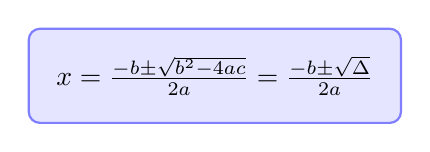
\begin{tikzpicture}
\node[rectangle, fill=blue!10, rounded corners, inner sep=10pt, draw=blue!50, thick] (box) {
$x = \frac{-b \pm \sqrt{b^2 - 4ac}}{2a} = \frac{-b \pm \sqrt{\Delta}}{2a}$
};
\end{tikzpicture}

\subsection*{Análise do Discriminante}
O discriminante $\Delta = b^2 - 4ac$ determina a natureza das raízes. Se $\Delta > 0$, existem duas raízes reais e distintas. Se $\Delta = 0$, existe uma raiz real dupla. Se $\Delta < 0$, não existem raízes reais (a parábola não toca o eixo $x$).

\subsection*{Exemplo}
Para $f(x) = x^2 - 5x + 6$, temos $a = 1$, $b = -5$, $c = 6$. Então $\Delta = (-5)^2 - 4(1)(6) = 25 - 24 = 1 > 0$. As raízes são:
\[
x = \frac{5 \pm \sqrt{1}}{2} = \frac{5 \pm 1}{2} \Rightarrow x_1 = 3 \text{ e } x_2 = 2
\]

% ============================================================
% SEÇÃO 3: VÉRTICE DA PARÁBOLA
% ============================================================
\section*{Vértice da Parábola}

\subsection*{Definição do Vértice}
O vértice é o ponto de máximo (se $a < 0$) ou mínimo (se $a > 0$) da parábola. É o ponto onde a função atinge seu valor extremo e coincide com o eixo de simetria.

\subsection*{Coordenadas do Vértice}
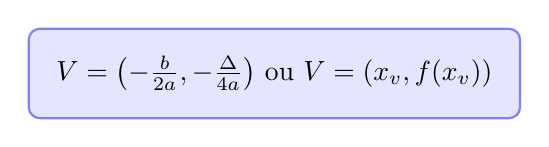
\begin{tikzpicture}
\node[rectangle, fill=blue!10, rounded corners, inner sep=10pt, draw=blue!50, thick] (box) {
$V = \left( -\frac{b}{2a}, -\frac{\Delta}{4a} \right)$ ou $V = \left( x_v, f(x_v) \right)$
};
\end{tikzpicture}

\subsection*{Significado Prático}
O vértice é fundamental para compreender o comportamento da função. Sua abscissa $x_v = -\frac{b}{2a}$ é o eixo de simetria da parábola. Sua ordenada $y_v$ representa o valor extremo (máximo ou mínimo) que a função assume.

\subsection*{Exemplo Prático}
Dada $f(x) = -2x^2 + 8x - 6$, temos $a = -2$, $b = 8$, $c = -6$. As coordenadas do vértice são:
\[
x_v = -\frac{8}{2(-2)} = 2, \quad y_v = f(2) = -2(4) + 8(2) - 6 = 2
\]
Logo, $V = (2, 2)$ é o ponto de máximo.

% ============================================================
% SEÇÃO 4: FORMA CANÔNICA E FATORADA
% ============================================================
\section*{Formas Alternativas da Função}

\subsection*{Forma Canônica}
A forma canônica (ou forma de vértice) é útil para identificar rapidamente o vértice:
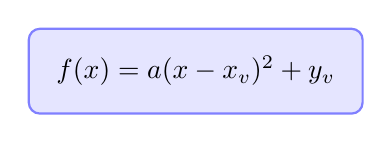
\begin{tikzpicture}
\node[rectangle, fill=blue!10, rounded corners, inner sep=10pt, draw=blue!50, thick] (box) {
$f(x) = a(x - x_v)^2 + y_v$
};
\end{tikzpicture}

\subsection*{Forma Fatorada}
Quando a função possui raízes reais $x_1$ e $x_2$, pode-se escrever:
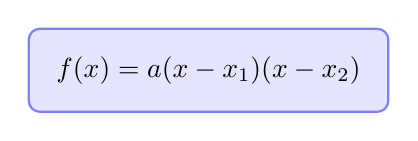
\begin{tikzpicture}
\node[rectangle, fill=blue!10, rounded corners, inner sep=10pt, draw=blue!50, thick] (box) {
$f(x) = a(x - x_1)(x - x_2)$
};
\end{tikzpicture}

\subsection*{Exemplo de Conversão}
A função $f(x) = x^2 - 6x + 8$ tem raízes $x_1 = 2$ e $x_2 = 4$. Sua forma fatorada é $f(x) = (x - 2)(x - 4)$.

% ============================================================
% SEÇÃO 5: SINAL DA FUNÇÃO
% ============================================================
\section*{Estudo do Sinal}

\subsection*{Análise de Positividade}
O estudo do sinal determina onde $f(x) > 0$ (positiva), $f(x) = 0$ (zero) e $f(x) < 0$ (negativa). Isso depende da concavidade da parábola e das raízes.

\subsection*{Casos Possíveis}
\begin{itemize}
\item Se $a > 0$ e $\Delta < 0$: $f(x) > 0$ para todo $x$ real
\item Se $a > 0$ e $\Delta = 0$: $f(x) \geq 0$ para todo $x$
\item Se $a > 0$ e $\Delta > 0$: $f(x) > 0$ se $x < x_1$ ou $x > x_2$; $f(x) < 0$ se $x_1 < x < x_2$
\item Se $a < 0$ e $\Delta < 0$: $f(x) < 0$ para todo $x$ real
\item Se $a < 0$ e $\Delta = 0$: $f(x) \leq 0$ para todo $x$
\item Se $a < 0$ e $\Delta > 0$: $f(x) < 0$ se $x < x_1$ ou $x > x_2$; $f(x) > 0$ se $x_1 < x < x_2$
\end{itemize}

% ============================================================
% SEÇÃO 6: EXERCÍCIOS BÁSICOS - RAÍZES
% ============================================================

\begin{enumerate}[leftmargin=*]

\section*{Atividade}
\item Calcule as raízes de $f(x) = x^2 - 7x + 12$.

\item Determine o discriminante de $f(x) = 2x^2 - 3x + 1$ e classifique as raízes.

\item Encontre as raízes de $f(x) = x^2 - 2x - 8$.

\item Qual é o valor de $\Delta$ para $f(x) = x^2 + x + 1$? A função possui raízes reais?

\item Resolva $3x^2 - 12x + 9 = 0$.

\end{enumerate}

% ============================================================
% SEÇÃO 7: EXERCÍCIOS - VÉRTICE
% ============================================================

\begin{enumerate}[leftmargin=*, start=6]

\item Calcule as coordenadas do vértice de $f(x) = x^2 - 4x + 3$.

\item Determine o vértice e diga se é máximo ou mínimo: $f(x) = -x^2 + 6x - 5$.

\begin{enumerate}[label=\alph*)]
\item Coordenadas do vértice
\item Classificação (máximo/mínimo)
\item Eixo de simetria
\end{enumerate}

\item Encontre o vértice de $f(x) = 2x^2 - 8x + 6$.

\item Qual é o valor máximo da função $f(x) = -3x^2 + 12x - 9$?

\item Para $f(x) = x^2 - 5x + 4$, determine a abscissa do vértice.

\end{enumerate}

% ============================================================
% SEÇÃO 8: EXERCÍCIOS - FORMA ALTERNATIVA
% ============================================================

\begin{enumerate}[leftmargin=*, start=11]

\item Converta $f(x) = (x - 3)(x + 2)$ para a forma geral.

\item Escreva $f(x) = x^2 - 6x + 8$ na forma fatorada.

\begin{enumerate}[label=\alph*)]
\item Identifique as raízes
\item Escreva a forma fatorada
\end{enumerate}

\item Transforme $f(x) = x^2 - 4x + 4$ na forma canônica.

\item Dada $f(x) = 2(x - 1)^2 - 3$ (forma canônica), identifique o vértice.

\item Expanda $(x - 2)^2 + 5$ para obter a forma geral.

\end{enumerate}

% ============================================================
% SEÇÃO 9: EXERCÍCIOS - SINAL E INEQUAÇÕES
% ============================================================

\begin{enumerate}[leftmargin=*, start=16]

\item Estude o sinal de $f(x) = x^2 - 5x + 6$.

\item Para quais valores de $x$ tem-se $x^2 - 4 > 0$?

\begin{enumerate}[label=\alph*)]
\item Encontre as raízes
\item Determine o sinal
\item Resolva a inequação
\end{enumerate}

\item Resolva a inequação $-x^2 + 4x - 3 \geq 0$.

\item Estude o sinal de $f(x) = 2x^2 - 8x + 8$.

\item Para que valores de $x$ temos $f(x) = x^2 - 2x - 3 < 0$?

\end{enumerate}

% ============================================================
% SEÇÃO 10: EXERCÍCIOS - APLICAÇÕES
% ============================================================

\begin{enumerate}[leftmargin=*, start=21]

\item Um projétil é lançado e sua altura é dada por $h(t) = -5t^2 + 20t$, onde $t$ é o tempo em segundos. Qual é a altura máxima atingida?

\item Uma empresa tem lucro dado por $L(x) = -2x^2 + 100x - 1200$, onde $x$ é a quantidade vendida. Determine a quantidade que maximiza o lucro.

\item Um terreno retangular tem perímetro de 40 metros. Se um lado mede $x$ metros, a área é $A(x) = x(20 - x)$. Qual é a área máxima?

\item A temperatura em uma cidade varia segundo $T(h) = -h^2 + 24h - 80$, onde $h$ é a hora do dia. Qual é a temperatura máxima?

\item Uma função de custo é $C(x) = x^2 - 10x + 50$. Qual é o custo mínimo?

\item O preço de um produto segue $P(x) = -2x^2 + 100x + 500$, onde $x$ é o mês. Em qual mês o preço é máximo?

\item A população de bactérias é $P(t) = -t^2 + 12t + 50$. Qual é a população máxima?

\item Um gráfico de receita é $R(x) = -3x^2 + 150x$. Qual quantidade maximiza a receita?

\item A altura de uma bola chutada é $h(t) = -10t^2 + 30t$. Após quanto tempo a bola retorna ao solo?

\item A eficiência de uma máquina é $E(x) = -x^2 + 8x - 12$. Qual é a eficiência máxima?

\end{enumerate}

\end{multicols}

\end{document}
